\chapter{Introduction}

The term network system passes on, an association of various PCs. For the most part, these systems have two kinds of availability, which are wired and remote. As on account of any innovation, it is development came out as a need. For any country, its most extreme need is to keep up military certainty. The first network system, was the beginning of the era and was essential set up in a military resistance venture called ARPANET, representing the Advanced Research Projects Agency Network. PC arranges throughout the years have developed a wide margin regarding highlights, intricacy, and power. Terms such as switches and routers are now recognizable to even the layman.

\vspace{5mm}
\section{Traditional Networks}

Even something as new and intense as network systems have demonstrated age. The maturing of innovation is by all accounts a lot snappier than people. Inside two decades, it built up an area of systems classified as traditional networks. Traditional networks are the spearheading plan of networks. Adam Smith of computer networking had a structure that was solid for the time and had no issues for quite a while. Indeed, even today, the traditional network system engineering cannot be blamed as is yet a subject of innovative work. Nevertheless, concerning each innovation that exists, there will be advantages and disadvantages.

\begin{figure}[!hbt]
    \centering
    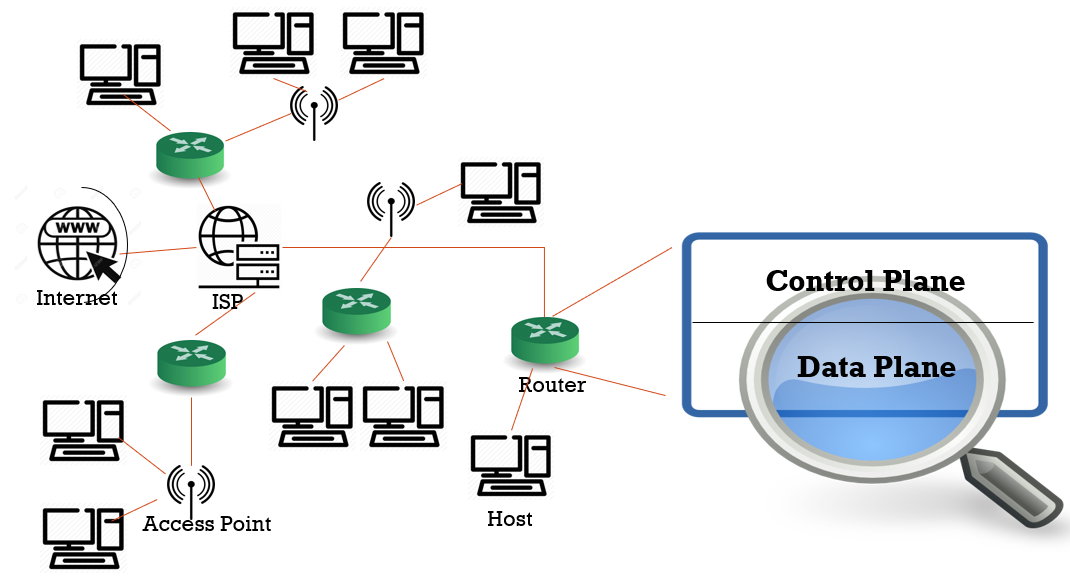
\includegraphics[width=\textwidth,keepaspectratio]{images/TRADITIONAL-NETWORK.png}
    \caption{Traditional Networks \cite{sdnimages}}
    \label{fig:Tradnets}
\end{figure}

   The computer network has been created for the sole purpose of communication. This means that digital information was transferred from one computer to another remote unit, through wire or air. It is equivalent to sending a post from one person to another. A letter was delivered to the post office, which redirects it to another post office, which will be nearest to the location of the recipient. 
    
    In the case of computer networks, this function of submitting a post is the same and is referred to as routing. No human intervention exists in computer networks; instead, there are independent computers responsible for transmitting this data. The task of routing is delegated to devices called routers, which today make up a fair share of the entire global network. 
    Routers play a vital role in today's network , i.e., forwarding packets through specific routes by identifying the current scenario of the neighboring devices and keeping track of the connected devices.  Similar to how someone seems to have a PO box connected to their location, every device in a local area network is listed under a router.  Such routers are dispersed across the network and are necessarily the foundation of the network.  The same explanation is that this method has heen tested for years in such a way that it has strong error detection and error correction. Such a network with millions of routing protocol devices ensures redundant information, so there is no single risk. 
    \vspace{2mm}
    
    This routing technique has been used for a long period of time. This will tend to be done for the lifespan of data networks. Across time, routing methods have improved significantly, and numerous techniques and network topologies \cite{topograph1996} have been researched and developed, rendering computer networks even more efficient in modern times. However, simply because something works well does not mean that it can not be improved. Although the debate is not regarding developing routing methods, in particular, it is stressed that the understanding of computer networks is so bland and outdated. The idea of transmitting a data packet with a header added to it to the enormous complexity of the global network appears to bind a message to a carrier pigeon and allow it to ride. Yeah, the pigeon knows how to reach the target by a step-by-step method, but neither the transmitter nor the receiver nor the network administrator knows where the packet is before it enters the informal network where either the recipient or the network administrator is constantly watching and hoping for the packet to arrive.
    
    A simple layout or architecture of the traditional network can be viewed from the Fig. \ref{fig:Tradnets}. There are several small networks connected to a common access point. These access-points are either switches, hubs, bridges or routers. These smaller networks are further connected to a common ISP, which gives these smaller networks access to the Internet.
    
   Packet forwarding is one aspect of the role of the network. Different highlights incorporate observing the system and checking which courses are accessible and which courses are down or under substantial loads with the goal that system traffic can be diverted to another course. Customary systems have some notable answers for such issues; huge numbers of them are ungainly and exploit the assumption that systems administration gadgets are because of quick preparing. They can manage numerous shortcomings simultaneously absent a lot of exertion. Although that might be real, it opens the path to change. Starting at now, there is no single controller to assess the exhibition of the huge system. The switches and routers deal with their immediate neighbours and assume that their neighbours can do likewise. At that point, it was a mind-blowing thought, yet it appears to be excessively simple.
        
    Another model of conventional systems is that every protocol, organize topology or design, expect that the whole network would run a solitary protocol for a lifetime. Then again, as it were, no protocol considered the requirement for versatility or similarity for change contingent upon the situation. A few conventions would adjust to deal with arrange inconsistencies and keep up reliable and unsurprising execution. In any case, the idea of making a network that could change its equipment and programming at some random time was unrealistic.
    
     On account of network issues, there are numerous measures sent to back up and ensure the system can be brought back ready for action. Be that as it may, the acknowledgement of network flaw over the whole network is excessively delayed as far as figuring speeds. In the event that one switch or a server fail someplace in this immense network, the mistake message from its neighbours needs some an ideal opportunity for it to get spread out and diffused to each other gadget in the system. This deferred reaction on account of system deficiencies is something that can be improved.
     
\section{Software Defined Networks}
    
    Traditional networks follow equipment hardware programming engineering. At the end of the day, the systems administration gadgets utilized, for instance, a switch, originated from a particular seller, and the merchant utilizes either their own exclusive programming on it or an outsider programming specially designed for their equipment. Rather, take the instance of a PC. It has equipment produced using a merchant, yet the equipment configuration permits us to introduce any working framework on it and utilize the framework in any methods. Some working frameworks offer more or preferable highlights over some others.
     The whole network has an equipment stage which is reasonable for any or different working frameworks one after another. The whole network isn't characterized by the equipment, rather than the working framework that sudden spikes in demand for it and deals with the system.
    
    Such a design as appeared in Fig. \ref{SDNArchitecure} is executed by adopting a concentrated network strategy on decentralized network engineering. The sentence seems like a confusing expression, however, its substance is to broaden the decentralized network engineering by keeping up the data forwarding techniques in its place and on the whole bringing together the system dynamic procedures into a legitimately single element. At the end of the day, the directing usefulness from the switches are evacuated, and they act as switches while making a central element to play out the routing choices and also screen the whole network. This element is named as ''Controller''. This postulation predominantly centres around controllers and the server where it is introduced.
    
    The Fig. \ref{SDNArchitecure} describes the layered architecture of SDN which has basically three distinct abstracted layers namely Application Plane (Application Layer), Control Plane (Control Layer) and Data Plane (Infrastructural Layer). To communicate between these layers, there is use of few APIs like North-Bound API which acts as an interface between Application Plane and Control Plane; South-Bound API acts as an interface between Control Plane and Data Plane. There is use of East-West Bound APIs which acts an interface between its and other Controller's Control Plane.
    
\begin{figure}[!hbt]
    \centering
     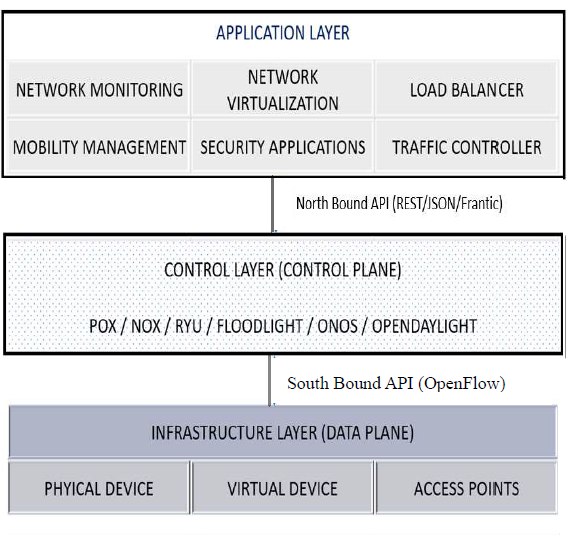
\includegraphics[width=10cm,keepaspectratio]{images/SDN-architecture-example.png}
    \caption{SDN Architecture \cite{sdnimages}}
    \label{SDNArchitecure}
\end{figure}

    Similar to Layer 1 or Physical Layer of OSI Model in Networking, the Infrastructural Layer or Data Plane of SDN Architecture has the main task is to transmit raw bits over a physical data link connected to various network nodes which can be implement either by using a physical or a virtual device. Addition to this, it also has  responsibility of Layer 2 or Data-Link Layer i.e. managing the communications links and handling frame traffic and govern a protocol to access the physical network medium. All these tasks are implemented by use of switches like OpenVSwitch.

    The Control Plane of SDN Architecture can be seen as the Layer 3 or Network Layer of OSI, which is  responsible for packet forwarding including routing through intermediate routers or other nodes. Unlike normal routers, the Control Plane of SDN is implemented at a server rather than on a router. The Control Plane features are established by use of a SDN Controller, an application. Some popular SDN Controllers are Pox, Ryu, Beacon, Nox, Floodlight, ONOS, OpenDayLight, Faucet, RunOS, etc. The Control Plane is also often termed as \textit{Network Operating System}.

    The Application Layer is the top most layer in SDN Architecture where several applications are installed on the server itself and run on top of Controllers via use of various North-Bound APIs build using REST, JSON, or similar languages. Tools like Load Balancers, Network Monitoring, Traffic Controllers, etc are some popular ones in the Application Layer.

    \textit{OpenFlow} is an open and standardized protocol and a flow-based switch specification, which acts as a South-Bound Interface in SDN. It is utilised for collaborating with the sending practices of switches from different merchants. It also control the behavior of switches throughput in a dynamic network and is also programmable. It helps to controller to communicate with switch over a secured channel. It also defines the format of packets.
    
    The corresponding switches are known as OpenFlow Switches. These switches has 3 parts namely an OpenFlow protocol, a flow table, and a secure channel. These switches has the responsibility to forward the flow's packets to given ports or, drop the flow packets or, forward the flow's packets to the controller by encapsulating it.

    As mentioned above, a divide and conquer approach is been followed in the SDN for networking tasks. \cite{taxonomy2014}. In place where every router in the network is performing both the tasks of routing and also of storing these routes to a routing table so to use these routes in future and also to notify the neighboring devices whenever there is a change in network which allows routers to focus on data-forwarding and this also reduces the repetitive calculations of find an optimal route. Whenever there is such new routes, the routers just need to ping the neighbours.
    
    All the functionality like calculation of optimal routes, screening of the topoloyg, or health of the network, are performed by the controllers. This helps to manage the entire network like an interface. This furthur brings in various benefits to the network The benefit of such a system is that there is no need to communicate the status of the network to the entire network. Instead, simply dump all information onto a central device or a collectively operating set of devices, and it will make sure that the network runs smoothly and in the most hassle-free manner.
     
    Another advantage of using a separate entity for controlling the network is that it allows the network to be protocol independent. In other words, the operating system or the software that is running on the controller is not fixed. The software-defined network architecture allows us to change the operating system whenever required \cite{arpanet2004}. Granted, it will be a time-consuming task before the network is up and running again, but it certainly is a quicker and cheaper alternative to having to change the software on all the devices in the network.

    In any technology, the rewards will always come at either a trade-off or at risk. From slow but convenient transportation of the bicycle to the spectacular but risky aviation technologies, development always comes at a cost.
    Similarly, in software-defined networking as well, there are some bills to be paid.
    
    Firstly the implementation of a collective entity called the controller is in the way of putting all eggs in one basket. This method, however efficient, still poses a risk. The general principle in any management technology is to increase redundancy. If, for a sizeable software-defined network, there is a single controller, in case of any faults ranging from power outages to natural disasters can cause the entire network to fail.  
    
    Another downside of software-defined networking is that the central controller does not necessarily monitor the actual traffic itself rather only the network's health and different routes. It does not necessarily monitor the traffic is because controllers are capable of monitoring network traffic using third-party applications. It is physically possible for the controller to continuously ping a switch in order to get the packets it handles and read its contents. However, it is incredibly impractical, and therefore pursuing such a feature would yield fewer returns than the effort put in. So naturally, developers do not focus on traffic monitoring as much as compared to network monitoring and routing. This significantly reduces the scope of software-defined networking as networks in which traffic cannot be monitored efficiently would pose a risk in terms of authenticity and privacy. Unless the entire network is trusted by the network administrator and the network participants, such a method would seem less preferred.
    
    Last but not least, as an extension to the points prior to the previous one, since a single entity controls the entire network's routing and monitors the network health and topology, this will obviously result in a severe overhead on the controller. It was mentioned that software-defined networks are operating system independent, but they are, in a way, dependent on the hardware limitations. Such as processing power, network bandwidth, and will prevent the network from growing beyond an absolute scale. As the network scales, so does the complexity in handling such an extensive network. Tasks such as routing, topology discovery \cite{netflow2004} become cumbersome unless the controller hardware is upgraded.
    
    Also, this makes the network elastic, meaning it tends to want to return to its original dimensions, due to overstress on the controller. Unless the controller device is changed, which, although not that expensive or time-consuming, generates a degree of unreliability in the network, in traditional networks, load balancing on routes would be performed by neighboring routers, and the task of network monitoring was delegated, this meant that the network overhead would never go beyond a limit. In case all the routers in the network reached its limit, merely adding more routers and breaking down large networks to smaller subnets would be enough. However, that is uncertain in the case of software-defined networks. Distributed controllers solve this problem to an extent, but still need more time to develop into a more robust approach.
    
    \section{Motivation \& Problem Statement}
    
    Software-Defined Networks brings a new perspective to network architectures. The concept of having a centralized approach to decentralized network architecture brings the merits of both architectures. SDN architecture provides the infrastructural flexibility and robustness of the traditional networks with the added feature of having a central interface to monitor and manage the entire network.
    
    There are many SDN implementations, each with a different controller operating system. However, there comes a question to choose the suitable controller for a network scenario where there are limited resources. Here, controllers are analyzed and tested for system-level performance metrics under a massive network traffic that appears similar to real-world networks. It helps to identify system-level bottlenecks of the controllers and makes it possible to classify controllers based on their system performances. It also generates the idea of whether the provided system is suited to a given controller and vice-versa.